\documentclass{elsarticle}

\usepackage{amsmath}
\usepackage{graphics}
\usepackage{graphicx}
\usepackage{color}
\usepackage{xspace}
\usepackage{url}
\usepackage[utf8]{inputenc}
\usepackage{booktabs}
\usepackage{caption}
\usepackage{subcaption}
\usepackage{epstopdf}

% reviews
\newcommand{\todo}[1]             {\textcolor{red}{[TODO] #1}}
\newcommand{\keoma}[1]            {\textcolor{blue}{[Keoma] #1}}
\newcommand{\remy}[1]             {\textcolor{blue}{[Remy] #1}}
\newcommand{\xavi}[1]             {\textcolor{blue}{[Xavi] #1}}
\newcommand{\thomas}[1]           {\textcolor{blue}{[Thomas] #1}}

 % lorem
\newcommand{\lorem}               {\textcolor{green}{Lorem ipsum dolor sit amet, consectetur adipisicing elit, sed do eiusmod tempor incididunt ut labore et dolore magna aliqua. Ut enim ad minim veniam, quis nostrud exercitation ullamco laboris nisi ut aliquip ex ea commodo consequat. Duis aute irure dolor in reprehenderit in voluptate velit esse cillum dolore eu fugiat nulla pariatur. Excepteur sint occaecat cupidatat non proident, sunt in culpa qui officia deserunt mollit anim id est laborum.}}

% shortcuts
\newcommand{\sm}                  {SmartMesh\xspace}
\newcommand{\smip}                {SmartMesh~IP\xspace}
\newcommand{\building}            {Smart Building\xspace}
\newcommand{\agri}                {Smart Agriculture\xspace}
\newcommand{\HRNEIGHBORS}         {{\tt HR\_NEIGHBORS}\xspace}
\newcommand{\HRDISCOVERED}        {{\tt HR\_DISCOVERED}\xspace}
\newcommand{\HRDEVICE}            {{\tt HR\_DEVICE}\xspace}
\newcommand{\pathcreate}          {{\tt path\_create}\xspace}
\newcommand{\pathdelete}          {{\tt path\_delete}\xspace}
\newcommand{\motecreate}          {{\tt mote\_create}\xspace}
\newcommand{\moteId}              {{\tt moteId}\xspace}
\newcommand{\PEACHNUMHRNEIGHBORS} {140,897\xspace}
\newcommand{\PEACHNUMSTATS}       {369,276\xspace}
\newcommand{\PEACHNUMPCKTS}       {693,844\xspace}
\newcommand{\EVANUMHRNEIGHBORS}   {128,072\xspace}
\newcommand{\EVANUMSTATS}         {386,929\xspace}
\newcommand{\EVANUMPCKTS}         {431,193\xspace}

\graphicspath{{figures/}}

\begin{document}

\begin{frontmatter}

\date{}

\title{Using \smip in \agri \\ and \building Deployments: it Just Works}

\author[inria]{Keoma~Brun-Laguna}
    \ead{keoma.brun@inria.fr}
\author[utn]{Ana~Laura~Diedrichs}
    \ead{ana.diedrichs@frm.utn.edu.ar}
\author[udp]{Diego~Dujovne}
    \ead{diego.dujovne@mail.udp.cl}
\author[utn]{Carlos~Taffernaberry}
    \ead{cartaffe@frm.utn.edu.ar}
\author[inria]{R\'emy~L\'eone}
    \ead{remy.leone@inria.fr}
\author[uoc]{Xavier~Vilajosana}
    \ead{xvilajosana@uoc.edu}
\author[inria]{Thomas~Watteyne}
    \ead{thomas.watteyne@inria.fr}

\address[inria]{~Inria, EVA team, Paris, France}
\address[utn]{~Universidad Tecnol\'ogica Nacional (UTN), Mendoza, Argentina}
\address[udp]{~Universidad Diego Portales, Santiago, Chile}
\address[uoc]{~Universitat Oberta de Catalunya, Barcelona, Catalonia, Spain}

\begin{abstract}
We deploy two low-power wireless networks, one in a \agri setting (a peach orchard), one in a \building.
Both networks use out-of-the-box \smip technology to gather sensor values, as well as extensive network statistics.
This article presents an in-depth analysis of the performance of both networks, and compares them.
Nodes in both exhibit end-to-end reliability of 100\%, with an expected lifetime between 4 and 8~years.
We show how -- contrary to popular belief -- wireless links are symmetric.
Thanks to the use of Time Slotted Channel Hopping (TSCH), the network topology is very stable, with $\leq$15 link changes on average per day in the entire 14-node network.
We conclude that \smip is a perfectly suitable IoT solution for \agri and \building applications.
\end{abstract}

\begin{keyword}
Low-power wireless, \smip, TSCH, 6TiSCH, \agri, \building.
\end{keyword}

\end{frontmatter}

%==============================================================================
\section{Introduction}
\label{sec:intro}

% agri: problem

Peaches do not like frost.
If during the blooming season (September in Argentina), temperature gets below $-$3~C for only a couple of hours, the flowers freeze, and no peaches are produced.
In 2013, 85\% of the peach production in the Mendoza region (Western Argentina) was lost because of frost events.
Farmers can lose everything in only a couple of hours.
Yet, if they are warned of a frost event a couple of hours ahead, they can install heaters throughout the orchard, and use big fans to move the hot air around.
Fighting the frost event is not the issue, what is hard is predicting them.

%======== front-page figure, do not move
\begin{figure}
    \centering
    \includegraphics[width=1.00\textwidth]{orchard}
    \caption{Devices deployed in a peach orchard near Mendoza, Argentina, for the \agri use case.}
    \label{fig:agri_pics}
\end{figure}

% agri: project

The goal of the \agri deployment (part of the PEACH~\cite{watteyne16peach} project) is to predict frost events in a peach orchard.
We install sensors around the orchard that measure air temperature, air relative humidity, soil moisture and soil temperature.
We feed the collected data into a database, and by analyzing the data in real-time using machine learning techniques, we can identify patterns in the data and predict frost events.

% agri: architecture

Because of the heavy machinery that moves inside the orchard, using cables to interconnect the sensors is not an option.
The main challenge is to deploy a system that provides both high end-to-end reliability and long lifetime, without using cables.
We use \smip off-the-shelf, the low-power wireless mesh solution from Analog Devices.
The sensor devices are battery-powered and equipped with a radio.
They form a multi-hop topology, and collaborate to route the data generated by the devices (called ``motes'') to a gateway.
This gateway is connected to the Internet, and forwards the gathered data to the servers in Paris, France.
Data appears on the web interface of the servers seconds after it was gathered by the sensor network.

% agri: deployment

The \agri network is deployed in a peach orchard of 204~trees, planted in a 50~m~$\times$~110~m area (shown in Fig.~\ref{fig:agri_map}).
The low-power wireless network is composed of 18~sensor motes uniformly distributed between the peach trees, and 3~relay motes to connect the orchard to the gateway some 300~m away.
Each mote is placed in a water-tight box that is fixed on a 4~m high pole (see Fig.~\ref{fig:agri_pics}).

\begin{figure}
    \centering
    \begin{subfigure}[h]{0.49\textwidth}
        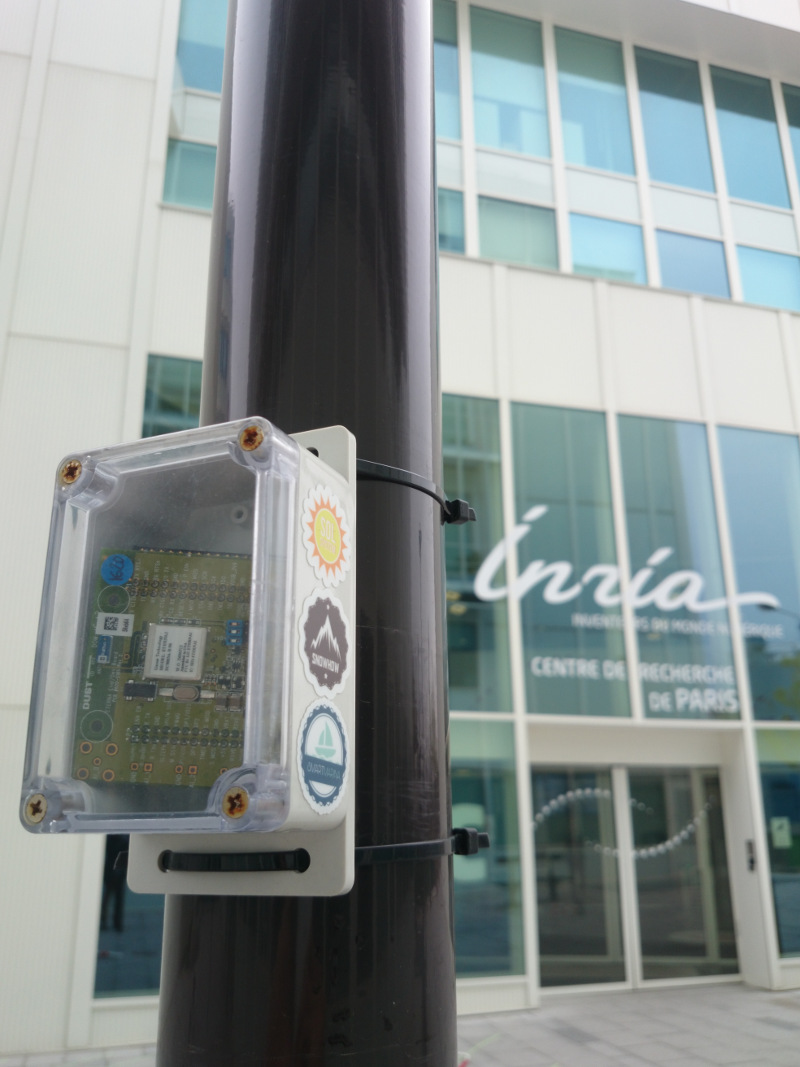
\includegraphics[width=\textwidth]{smartbuilding_outdoor}
        \caption{outdoors}
    \end{subfigure}
    \begin{subfigure}[h]{0.49\textwidth}  
        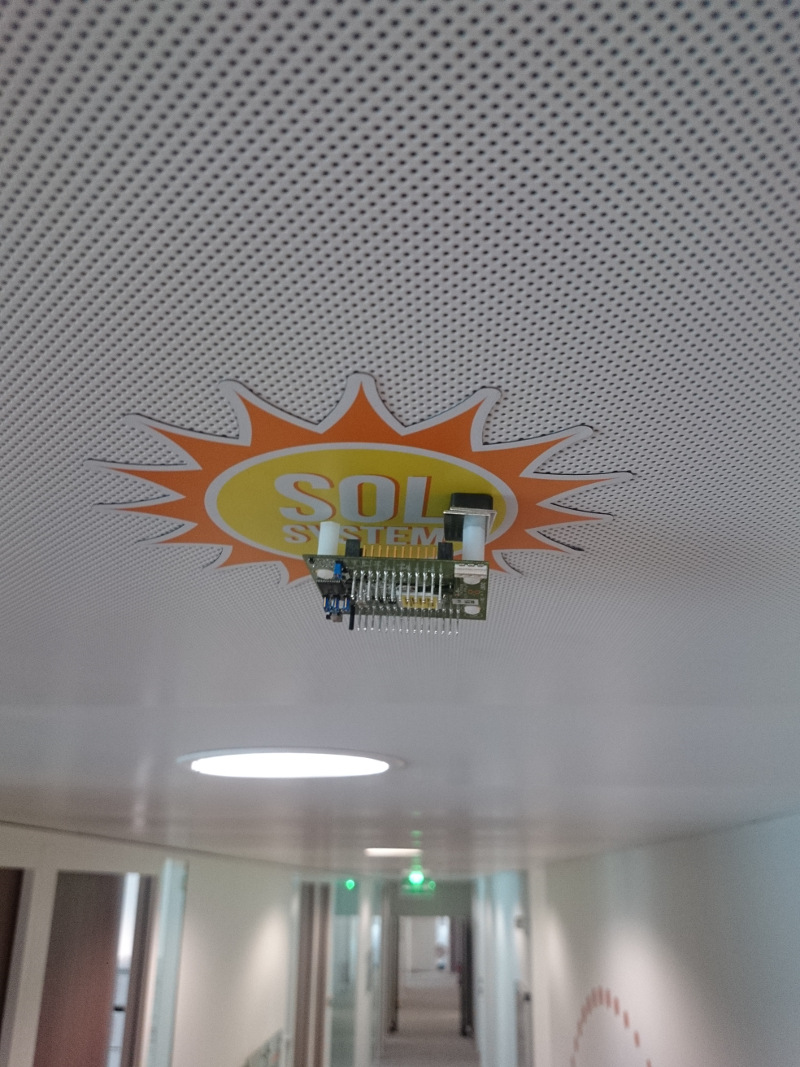
\includegraphics[width=\textwidth]{smartbuilding_indoor}
        \caption{indoors}
    \end{subfigure} 
    \caption{Devices deployed in the Inria-Paris offices for the \building use case.}
    \label{fig:building_pics}
\end{figure}

% building: deployment

To complement and compare the network performance gathered from the \agri deployment, we deploy a second \building low-power wireless network in an office building in Paris, France.
14~motes are placed on the ceiling of one floor of the building, 3~additional motes are placed right outside the building, on lamp posts (Fig.~\ref{fig:building_map}).
The 14~motes inside are fixed to the ceiling using magnets; the 3~motes outside are placed in a water-tight boxes (Fig.~\ref{fig:building_pics}).
Thanks to the ``peel-and-stick'' nature of this low-power wireless technology, deployment takes less than an hour.

% hardware

In the \agri deployment, we use four types of \smip devices.
Inside the orchard, 2~DC9018 boards feature an external antenna, 16~DC9003 boards a chip antenna.
We deploy 3~long-range repeaters outside the orchards to connect the network to the gateway, located some 300~m away.
In the \building deployment, we use 2 types of \smip devices: 11~DC9003 boards (chip antenna), 1~DC9018 board (external antenna).
For both deployments, the gateway is composed of a Raspberry~Pi single-board computer connected to a DC2274 \smip manager over USB.
All boards are off-the-shelf, manufactured by Analog Devices.

% technology

\smip is a product line developed by the Dust Networks Product Group at Analog Devices.
The \smip network stack is based on 6LowPAN and the 802.15.4e standards and provides an API for the user to write applications.
The \smip network implements the IEEE802.15.4 TSCH mode~\cite{std_ieee802154_2015}, which includes a channel-hopping mechanism to reduce the impact of multi-path fading and external interference.
This allows the network to be highly reliable, stable, and extremely low power~\cite{watteyne10mitigating,watteyne09reliability}.
We use the default application where each mote produces a temperature value every 30~s, and network statistics every 5~min.
We extract 3~months of data for each deployment, resulting in over 4~million temperature values, and more than 350,000~network statistic measurements for each deployment.

\begin{figure}
    \centering
    \begin{subfigure}[h]{0.70\textwidth}
        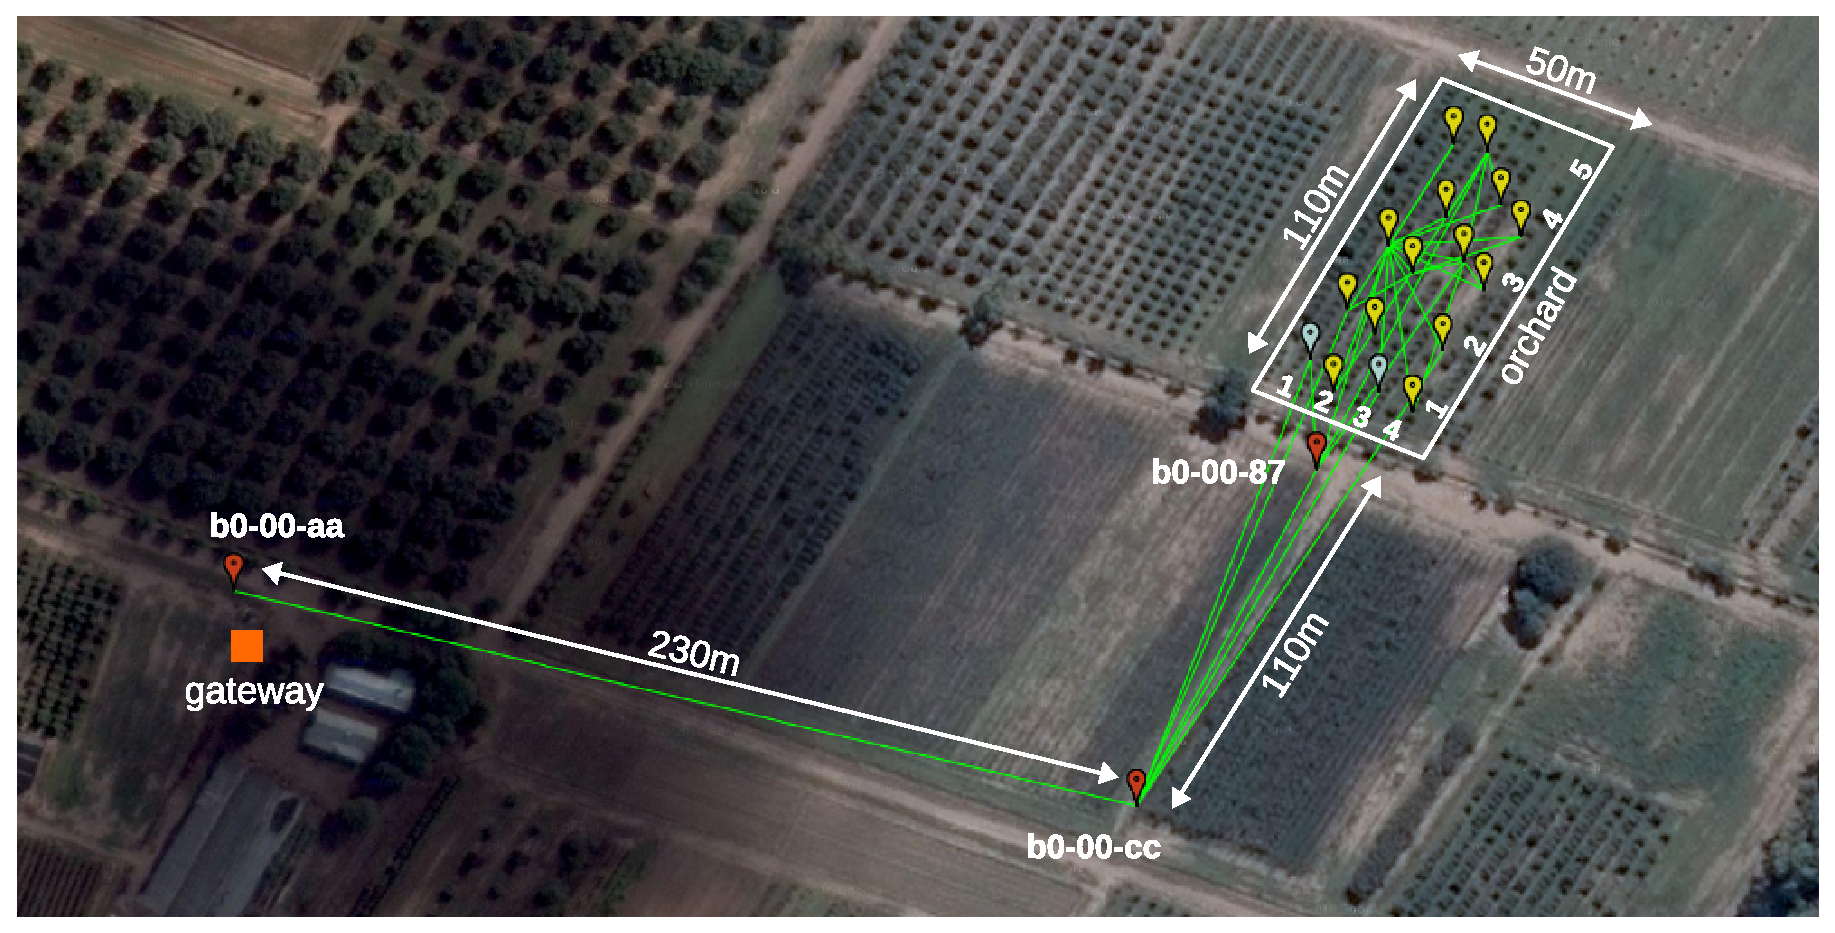
\includegraphics[width=\textwidth]{map_annotated}
        \caption{\agri}
        \label{fig:agri_map}
    \end{subfigure}
    \begin{subfigure}[h]{0.27\textwidth}  
        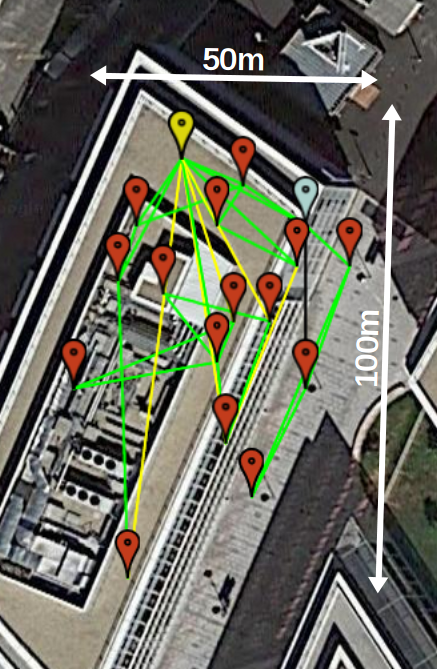
\includegraphics[width=\textwidth]{evalab_map_annotated}
        \caption{\building}
        \label{fig:building_map}
    \end{subfigure} 
    \caption{
        Aerial view of the topology of both deployments.
        The deployment is done in both cases in a roughly 50~m~$\times$~100~m area.
    }
    \label{fig:maps}
\end{figure}

% goal of this article

The goal of this article is to analyze the network statistics over each of the 3-month periods, precisely assess the performance of both networks, and contrast/compare them.
This article makes the following contributions:

\begin{itemize}
    \item We confirm that the \smip network exhibits years of battery lifetime and wire-like reliability in both cases;
    \item We show that channel hopping causes the network topology to be very stable, with $\leq$15 link changes on average per day on the 14-node and 18-node networks;
    \item Contrary to popular belief, we show that links in the networks are symmetric, i.e.~they exhibit the same signal strength in both directions of the same link;
    \item We conclude that \smip is a perfectly suitable IoT solution for \agri and \building applications.
\end{itemize}

% extension

This article in an extension of a previously published paper~\cite{brun16intuitive}, which only presented results for the \agri deployment, over a 3-week period.
This article offers analysis over a 3-month period, and contrasts and compares the performance of \smip in the \agri deployment with that in a (new) \building deployment.

% remainder

The remainder of this article is organized as follows.
Section~\ref{sec:collected} describes the types of network statistics, and the dataset of statistics collected over each 3~month periods.
Section~\ref{sec:intuitive} presents results that confirm assumptions about what we can expect for a real-world \smip deployment.
Section~\ref{sec:notsointuitive} presents not so intuitive results about link symmetry and network stability.
Finally, Section~\ref{sec:conclusion} concludes this article and discusses further improvements.

%==============================================================================
\section{Statistics Collected}
\label{sec:collected}

% environment

The \agri network is deployed in a peach orchard in Jun\'in, 45~km South-East of Mendoza in Western Argentina.
No other electronic devices are present in the field.
Farmers work inside the field with heavy machinery for 1-2~h every 20~days approximately.
In the region, air temperature ranges between $-$9~C in winter (May-October) to +38~C in summer (November-April).
Because of the sunny weather, day/night temperature swings of 10+~C are not uncommon in winter.

The \building network is deployed in the Inria-Paris offices (a research institute) in Paris, France.
It is deployed in a typical 5-story office building, in which light-material walls separate offices which are arranged around a concrete core which houses the elevators.
Several wireless technologies operate in the same building, including Wi-Fi, Bluetooth and other IEEE802.15.4-based networks.
Around 200~people work in that building, with lots of activity, mainly during business hours.

% events and HR

Each device in the network produces both sensor data and network statistics.
Network statistics can be separated in Events and Health Reports messages.
\textit{Event} messages are non-periodic notifications the network sends when a network event happens (e.g.~a mote joins/leaves the network, a link is created/deleted).
\textit{Health Report} (HR) messages are sent periodically by each mote; they contain counters and statistics about that mote.
HRs are used to assess the health and performance of the network.

% number received and remainder

\begin{table}
    \centering
    \begin{tabular}{|l|r|r|}
        \toprule
        \multicolumn{1}{|c|}{type} & \multicolumn{1}{|c|}{\agri} & \multicolumn{1}{|c|}{\building} \\ \hline
        \hline
        \motecreate                &                         133 &                              85 \\ \hline
        \pathcreate                &                       4,098 &                           1,403 \\ \hline
        \pathdelete                &                       3,653 &                           1,325 \\ \hline
        \HRDEVICE                  &                     132,758 &                         154,698 \\ \hline
        \HRDISCOVERED              &                      87,737 &                         152,641 \\ \hline
        \HRNEIGHBORS               &        \PEACHNUMHRNEIGHBORS &              \EVANUMHRNEIGHBORS \\ \hline
    \end{tabular}
    \caption{The number of statistics collected over the 3~month periods.}
    \label{tab:msg_stats}
\end{table}

Table~\ref{tab:msg_stats} summarizes the number of events and HRs gathered during the 3~month periods of both deployments:

\begin{itemize}
    \item[-] \textbf{\motecreate.}
        Each node in a \smip network periodically sends beacons to announce the presence of the network.
        When a mote wants to join a network, it listens for those beacons.
        Once it has heard a beacon, the new mote starts a security handshake with the network.
        During that handshake, the \smip manager sends a \motecreate event notification over its serial port.
        This is the event we log\footnote{~Normally, each mote generates a single \motecreate event. Due to power issues at the manager side, the network restarted a couple of times and new events were created.}.
        It contains, among other information, the association between the newly-joined device's 8-byte MAC address and its 2-byte \moteId.
    \item[-] \textbf{\pathcreate} and \textbf{\pathdelete.}
        In \smip terminology, a ``path'' is the link-layer resource that allows two neighbor nodes to communicate\footnote{~In more classical networking terminology, this is often referred to as a ``link''. We use the terms ``path'' and ``link'' interchangeably in this article.}.
        Each time a mote starts communicating with a new neighbor (e.g.~its routing parent), a \pathcreate event is produced.
        Similarly, each time a mote \textit{stops} communicating with a neighbor (e.g.~it changes routing parent), a \pathdelete event is produced.
        We log both messages.
    \item[-] \textbf{\HRDEVICE.}
        Each network device produces a \HRDEVICE every 15~min.
        This health report contains counters/statistics internal to the mote, such as its current battery voltage, temperature, or total number of messages sent.
    \item[-] \textbf{\HRDISCOVERED.}
        \sm nodes continuously monitor their surroundings to discover neighbor nodes.
        Every 15~min, each node produces an \HRDISCOVERED health report that contains the list of ``discovered'' neighbors, and the associate signal strength it heard them at.
        These discovered neighbors can potentially be used in the future as neighbors the node communicates with.
    \item[-] \textbf{\HRNEIGHBORS.}
        Two nodes are neighbors when link-layer resources are installed for them to communicate.
        The neighbors of a node are a subset of the discovered neighbors.
        Every 15~min, each note generates an \HRNEIGHBORS health report that contains its list of neighbors.
        These messages also specifies per-neighbor counters, such as the number of link-layer retransmissions.
\end{itemize}

% analysis

After 3~months of operation, we have collected \PEACHNUMSTATS and \EVANUMSTATS network statistics in the \agri and \building deployment, respectively (see Table~\ref{tab:msg_stats}).
The goal of the next section is to present the main results from analyzing this information.
We group these results in two categories.
``Intuitive'' results (Section~\ref{sec:intuitive}) are results that confirm the performance expected from a \smip network.
``Not so intuitive'' results (Section~\ref{sec:notsointuitive}) are results that we believe go against popular belief.
This classification is necessarily subjective.

Due to power line failure at the network manager side, the network experienced several restarts.
For this reason, some analysis presented in the next sections are done in shorter period.
As a beneficial side effect, this allows us to verify the network formation and joining process.

%==============================================================================
\section{Intuitive Results}
\label{sec:intuitive}

% intro

Previous publications~\cite{watteyne16peach,watteyne10mitigating,watteyne09reliability,watteyne15industrial} underline the performance of TSCH networks in general, and \smip in particular.
Standardization work in the IETF 6TiSCH working group\footnote{~\url{https://datatracker.ietf.org/wg/6tisch/about/}} around TSCH networks further illustrates the move of the industry towards this type of networking technology.
While we generally expect good performance from the network, this section verifies that this is the case, on the commercial \smip implementation.

% remainder

We start by looking at two physical-layer metrics: RSSI vs Distance (Section~\ref{sec:rssi_distance}) and PDR vs. RSSI (Section~\ref{sec:waterfall}).
While these have no dependency on TSCH (the type of medium access), they allow us to verify the overall connectivity in the network.
We then look at key performance indicators: end-to-end reliability (Section~\ref{sec:net_reliability}) and network lifetime (Section~\ref{sec:lifetime}).

%------------------------------------------------------------------------------
\subsection{RSSI vs. Distance}
\label{sec:rssi_distance}

The Friis transmission model~\cite{saunders07antennas} gives the relationship between the Received Signal Strength (RSSI)\footnote{~Strictly speaking, the RSSI is the Received Signal Strength \textit{Indicator}, a value returned by the radio chip. Because of its prevalence in low-power wireless literature, we use RSS and RSSI interchangeably.} in free space.
While the Friis transmission model  does \textit{not} apply directly to our real-world deployment, we note in Fig.~\ref{fig:pister_hack} that the individual RSSI values are located between the Friis model, and the Friis model offset by $-$40~dB.
This corroborates the results from~\cite{zats10wireless}.

\begin{figure}
    \centering
    \begin{subfigure}[h]{0.49\textwidth}
        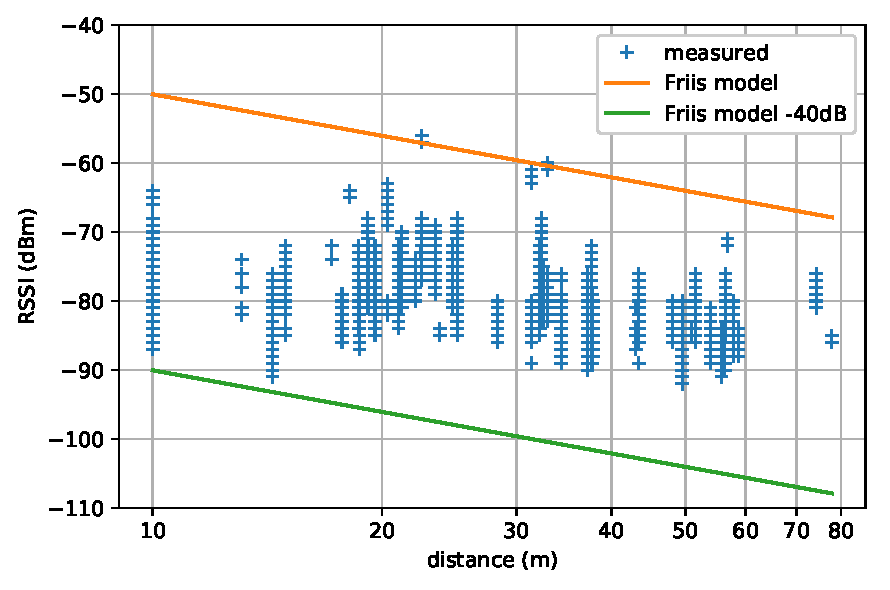
\includegraphics[width=\textwidth]{pister_hack_agri.eps}
        \caption{\agri}
    \end{subfigure}
    \begin{subfigure}[h]{0.49\textwidth}  
        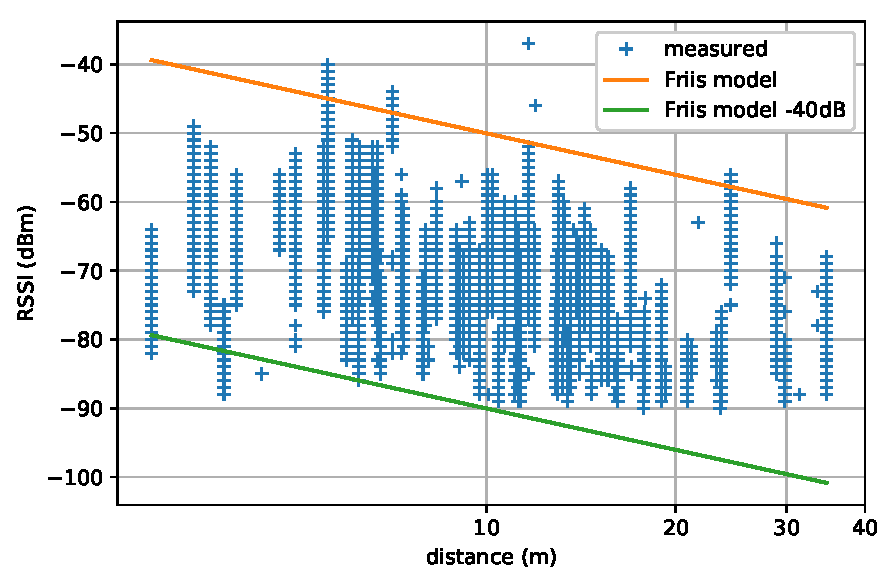
\includegraphics[width=\textwidth]{pister_hack_building.eps}
        \caption{\building}
    \end{subfigure} 
    \caption{RSSI measurements are roughly located between the Friis model and the Friis model shifted by $-$40~dB.}
    \label{fig:pister_hack}
\end{figure}

%------------------------------------------------------------------------------
\subsection{Wireless Waterfall}
\label{sec:waterfall}

% sample presentation

Due to the inherent physical unreliability of the radio medium, it is impossible to know if a future transmission will succeed or not.
The Packet Delivery Ratio (PDR) is the portion of successful link-layer transmissions over the total number of link-layer transmission attempts.
A failed attempt means that the link-layer frame needs to be re-transmitted; this does \textit{not} mean the packet is lost.
Over a period of 3~months, \PEACHNUMHRNEIGHBORS~\HRNEIGHBORS messages are collected in the \agri deployment and \EVANUMHRNEIGHBORS in the \building deployment.
These contain, for a given node, the number of link-layer transmission attempts and successes to each of its neighbors.
We remove the portion of neighbors with no transmission and keep only the DC9003 motes, resulting in a total of 69,643 messages (approx. 49\% from the total number of \HRNEIGHBORS) for the \agri deployment and a total of 93,135 messages (approx. 73\%) for the \building deployment.

% plot

Fig.~\ref{fig:waterfall} plots the PDR and the RSSI of these 69,643 and 93,135 messages.
For readability, we also plot the average/deviation of the data for a given RSSI value.
Because of its shape, this is known as the ``waterfall plot''.

\begin{figure}
    \centering
    \begin{subfigure}[h]{0.49\textwidth}
        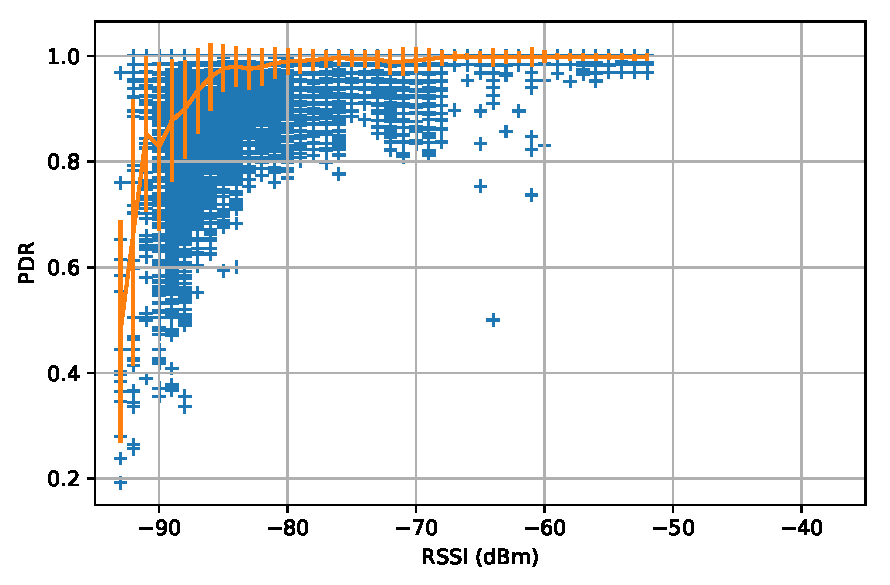
\includegraphics[width=\columnwidth]{waterfall_agri}
        \caption{\agri}
        \label{fig:waterfall_agri}
     \end{subfigure}
     \begin{subfigure}[h]{0.49\textwidth} 
        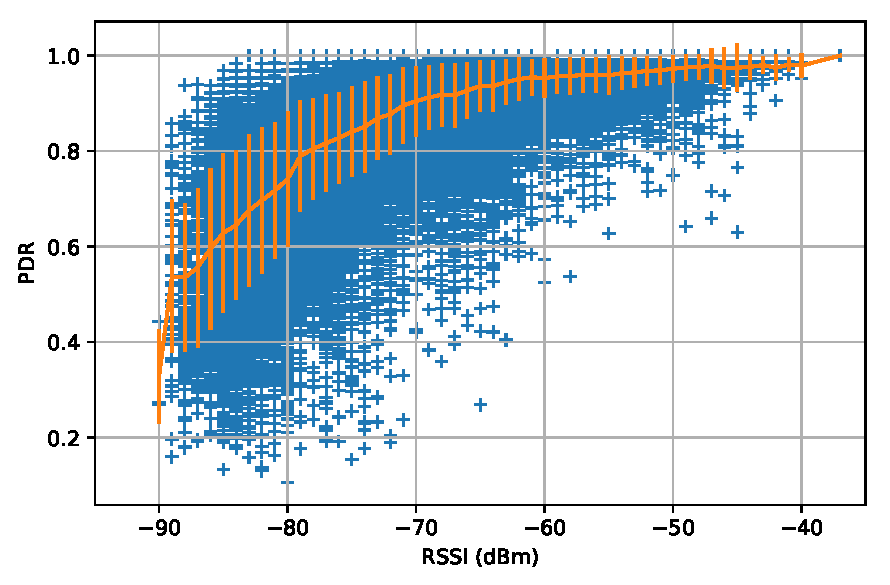
\includegraphics[width=\columnwidth]{waterfall_building}
        \caption{\building}
        \label{fig:waterfall_building}
    \end{subfigure}
    \caption{
        The PDR/RSSI ``waterfall'' plot.
        The \building plot is shifted right compared to the \agri plot, indicating an environment where external interference is present.
    }
    \label{fig:waterfall}
\end{figure}

For the \agri deployment, the average PDR of the links is very good~($>95$\%) above $-85~dBm$.
Below that value, the PDR rapidly degrades, indicating that, on these links, frequent retransmissions happen.
For the \building deployment, the PDR starts to degrade at $-60~dBm$.
Note that, if the network were using a non-schedule MAC layer (e.g.~ZigBee), the PDR for the same RSSI would be lower than in Fig.~\ref{fig:waterfall} because of collisions.
The device manufacturer documentation~\cite{smip_app_note} indicates that a path is considered as ``bad'' when:

\begin{itemize}
    \item RSSI$>-80~dBm$ and PDR$<50$\%
    \item RSSI$>-70~dBm$ and PDR$<70$\%
\end{itemize}

This is not the case in any of the two deployments.

% interferences

The waterfall plot allows us to assess the level of external interference.
In the presence of external interference, the waterfall plot is either shifted to the right with very few paths below $-70~dBm$, or does no constantly increase with RSSI.

The waterfall plot in the \agri deployment (Fig.~\ref{fig:waterfall_agri}) is ``clean'', meaning that the \smip network is not experiencing high levels of external interferences from co-located wireless devices.
Especially when comparing both, the waterfall plot in the \building deployment \textit{is} shifted to the right (Fig.~\ref{fig:waterfall_agri}), indicating the \smip network is experiencing external interferences.
This is expected, as several hundred WiFi devices and tens of WiFi access points are operating in the building.
Yet, despite the high external interfere, the \building deployment exhibits 100\% end-to-end reliability (as detailed in Section~\ref{sec:net_reliability}), underlying the resiliency of \smip to external interference.

%------------------------------------------------------------------------------
\subsection{End-to-End Reliability}
\label{sec:net_reliability}

% steady state results

We expect the \smip network to offer wire-like reliability.
Table~\ref{tab:net_stats} confirms that this is the case.
It presents statistics gathered over the 15-25 July 2016 period in the \agri deployment, and over the 12 November 2016 - 12 February 2017 period in the \building deployment.
Both sensor data and network statistics are taken into account.

\begin{table}
    \centering
    \begin{tabular}{|l|r|r|}
        \toprule
        {}                              & \agri                     & \building                    \\
        \midrule
        reliability                     & \textbf{100\%}            & \textbf{100\%}               \\
        (Arrived/Lost)                  & (\PEACHNUMPCKTS~/~0)      & (\EVANUMPCKTS~/~0)           \\
        \hline
        average PDR                     & 95\%                      &  87\%                        \\
        (Transmit/Fails)                & (4,405,569~/~258,778)     &  (19,807,535~/~2,488,149)    \\
        \hline
        latency                         & 700~msec                  &  \textit{not measured.}      \\
        \bottomrule
    \end{tabular}
    \caption{The overall network performance in the 15-25 July 2016 period (\agri) and the 12 Nov. 2016 - 12 Feb. 2017 period (\building).}
    \label{tab:net_stats}
\end{table}

It shows that, as none of the \PEACHNUMPCKTS and \EVANUMPCKTS packets generated in the networks was lost, the end-to-end reliability is 100\%.
The average PDR over all links is very high (95\% and 87\%), indicating that the nodes are deployed close enough to one another.
Finally, the average latency over all nodes is 700~ms for the \agri deployment.
These results are very similar to the very initial results presented in~\cite{watteyne16peach}, indicating \textit{no} degradation in performance of the \smip network over the 3~month periods.

%------------------------------------------------------------------------------
\subsection{Network Lifetime}
\label{sec:lifetime}

% description

Each device is powered by a pair of Energizer L-91 AA batteries\footnote{http://data.energizer.com/pdfs/l91.pdf}.
These contain a nominal 3134~mAh of charge, or 2821~mAh when accounting for a 10\% decrease due to manufacturing differences.
A \smip node contains a ``charge accounting'' feature in which it tracks the amount of charge it has been drawing from the battery.
Each mote reports this number every 15~min as a field in its \HRDEVICE health report.
This number allows us to predict the lifetime of the device.

% results

Table~\ref{tab:stats_charge} shows charge consumed by the motes over the two 3~month periods.
Assuming a relatively constant energy consumption rate, we extrapolate the lifetime.
The nodes with the longest lifetime (8~years) are all leaf nodes as we can see from Fig.~\ref{fig:maps}.
Since they do not have to relay data from any children, it is expected for these motes to consume the least.
The mote with the shortest lifetime is {\tt 30-60-ef}, with a 4~year battery lifetime.
This is expected, as this mote relays an important amount of data.
This confirms the ultra-low power consumption of the \smip network.

\begin{table}
\begin{subtable}{.5\textwidth}
    \begin{tabular}{|c|c|r|}
        \toprule
        MAC           &  charge  & lifetime \\
                      & consumed$^\star$ &          \\
        \midrule
        \tt{30-60-ef} &          695 KC &  4 years \\
        \tt{38-0f-66} &          461 KC &  6 years \\
        \tt{3f-f8-20} &          380 KC &  8 years \\
        \tt{3f-fe-87} &          549 KC &  5 years \\
        \tt{3f-fe-88} &          718 KC &  4 years \\
        \tt{58-32-36} &          311 KC &  7 years \\
        \tt{60-01-f8} &          387 KC &  8 years \\
        \tt{60-02-1b} &          371 KC &  8 years \\
        \tt{60-02-4b} &          406 KC &  7 years \\
        \tt{60-03-82} &          395 KC &  8 years \\
        \tt{60-05-5f} &          386 KC &  8 years \\
        \tt{60-05-69} &          509 KC &  6 years \\
        \tt{60-05-78} &          364 KC &  8 years \\
        \tt{60-05-ab} &          381 KC &  8 years \\
        \tt{60-06-27} &          422 KC &  7 years \\
        \tt{60-08-d5} &          432 KC &  7 years \\
        \bottomrule
    \end{tabular}
    \caption{\agri}
\end{subtable}\hfill
\begin{subtable}{.43\textwidth}
    \begin{tabular}{|c|c|c|}
        \toprule
        MAC           &  charge  & lifetime \\
                      & consumed$^\star$ &          \\
        \midrule
        \tt{38-03-dd} &          459 KC &  5 years \\
        \tt{58-e9-ca} &          411 KC &  6 years \\
        \tt{58-e9-cb} &          407 KC &  6 years \\
        \tt{58-eb-5b} &          423 KC &  6 years \\
        \tt{58-eb-64} &          322 KC &  8 years \\
        \tt{58-eb-67} &          468 KC &  5 years \\
        \tt{58-eb-69} &          243 KC &  7 years \\
        \tt{58-f3-17} &          357 KC &  7 years \\
        \tt{58-f4-f8} &          402 KC &  6 years \\
        \tt{58-f5-23} &          416 KC &  6 years \\
        \tt{58-f5-3c} &          412 KC &  6 years \\
        \tt{58-f5-58} &          387 KC &  6 years \\
        \tt{58-f8-63} &          198 KC &  9 years \\
        \tt{58-f8-78} &          233 KC &  7 years \\
        \tt{58-f8-8f} &          439 KC &  6 years \\
        \tt{58-f9-c4} &          325 KC &  8 years \\
        \bottomrule
    \end{tabular}
    \caption{\building}
\end{subtable}\hfill
\vspace{2mm}
$^\star$~over the 3.5 months and 3 months periods respectively.
\caption{Per-node power consumption and associated expected lifetime when powered by a pair of AA batteries.}
\label{tab:stats_charge}
\end{table}

%==============================================================================
\section{Not so Intuitive Results}
\label{sec:notsointuitive}

Results from Section~\ref{sec:intuitive} are ``intuitive'' is that they corroborate previous measurements~\cite{watteyne16peach} or confirm theoretical/lab results~\cite{watteyne10mitigating,watteyne09reliability,watteyne15industrial}.
This section presents results which we believe go against popular belief.
This classification is necessarily subjective.

In Section~\ref{sec:symmetry}, we show that links are, in fact, symmetric.
In Section~\ref{sec:net_stability}, we show that, through the use of TSCH, the low-power wireless topology is, in fact, extremely stable.

%------------------------------------------------------------------------------
\subsection{Link (A)Symmetry}
\label{sec:symmetry}

% what is reported

Motes report the average RSSI value of the packets received from each neighbor in their \HRNEIGHBORS health reports.
Because the network uses channel hopping, the reported RSSI values are also averaged over 15~IEEE802.15.4 frequencies~\cite{std_ieee802154_2015}.
In this section, we use the term ``RSSI'' to denote the average RSSI over 15 frequencies.

% what is asymmetry

A common assumption is that links between neighbor low-power wireless devices are hugely asymmetric.
That is, on a link between nodes $A$ and $B$, $A$ receives $B$'s link-layer frames with an RSSI very different from the frames $B$ receives from $A$.
Numerous routing protocols (often standardized~\cite{rfc3626}) reuse that assumption and start with a costly step of filtering out asymmetric links.

% what we measure

We look at the link statistics between 18 June 2016 and 4 July 2016 (16 days) in the \agri deployment, and between the 12 November 2016 and 7 February 2017 (87 days) in the \building deployment.
The sample contains 411,132 \HRNEIGHBORS messages received from 14~DC9003 nodes (same hardware).
During that period, 21~links are active with at least 250~transmissions for each link.
For each of those links, we compute the difference between average RSSI in each directions.
Results are presented in Fig.~\ref{fig:tab_symmetry}.

\begin{figure}
    \centering
    \begin{subfigure}[h]{0.49\textwidth}
        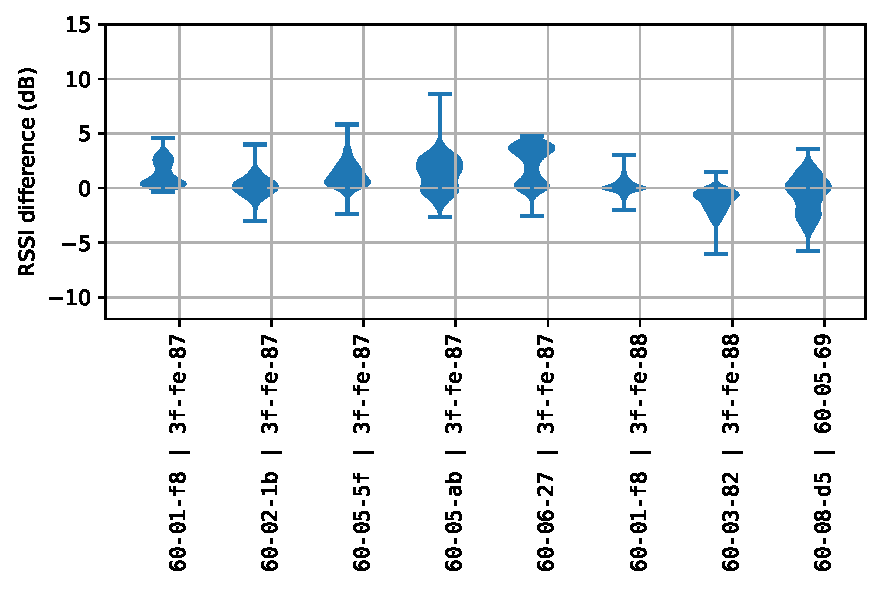
\includegraphics[width=\columnwidth]{asymmetry_agri.eps}
        \caption{\agri}
    \end{subfigure}
    \centering
    \begin{subfigure}[h]{0.49\textwidth}
         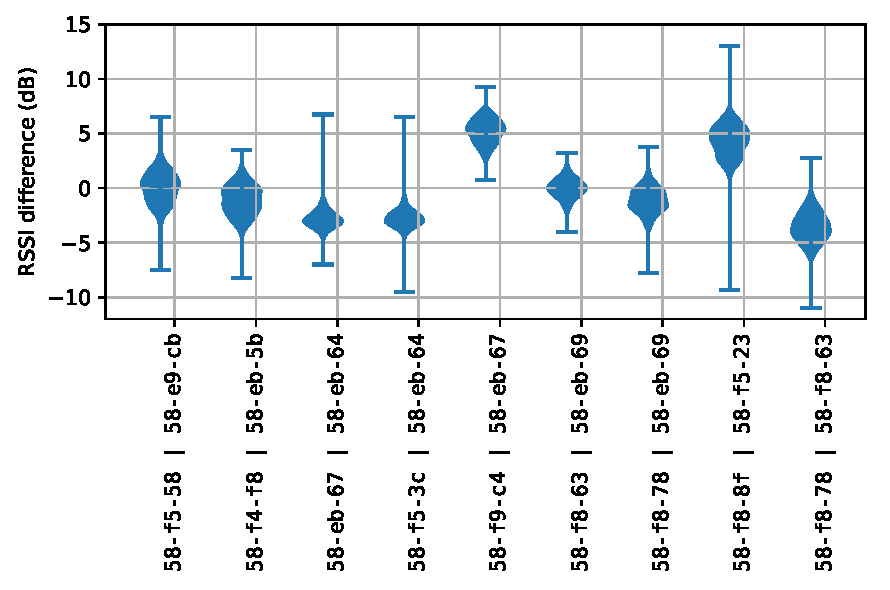
\includegraphics[width=\columnwidth]{asymmetry_building.eps}
        \caption{\building}
    \end{subfigure}
    \caption{
        The difference in RSSI between the two directions of the wireless links with the highest number of exchanged messages.
        The violin plots show the distribution of the value and the standard deviation.
    }
    \label{fig:tab_symmetry}
\end{figure}

% discussion

Fig.~\ref{fig:tab_symmetry} shows that the RSSI difference never exceeds a couple of dB.
Looking at Fig.~\ref{fig:waterfall}, this translates into only a handful of percentage points difference in PDR.
This means the links can be considered symmetric.
This result is in-line with the physical phenomenon that the signal traveling from $A$ to $B$ undergoes the same attenuation as that from $B$ to $A$.
This result would \textit{not} hold if the neighbor radios had a different transmit power or sensitivity.
That being said, discussions on link symmetry at the routing layer is largely artificial, as virtual all state-of-the-art medium access control (MAC) protocols uses link-layer acknowledgments.

%------------------------------------------------------------------------------
\subsection{Network Stability}
\label{sec:net_stability}

% unreliability

Wireless in unreliable in nature.
It is normal that some wireless links interconnecting motes ``come and go''.
That is, links that have been performing well (e.g.~PDR$>$90\%) can suddenly disappear (e.g.~PDR$<$10\%).
Similarly, nodes that were not able to communicate can suddenly hear one another perfectly.

% time scale

The question, however, is what time scale is considered.
Early academic work on low-power wireless~\cite{srinivasan08beta} has looked at the ``burstiness'' of the wireless links, i.e.~changes over the course of 10-1000's~ms.
Some follow-up work has taken the assumption that wireless links are so unstable that only a reactive routing approach works.
In this section, we infirm this statement by looking at the stability of the network.

% dataset

In particular, we look at the \pathdelete and \pathcreate events.
These are generated each time a node adds/deletes a neighbor to communicate with, which happens for example when the routing topology changes (see Section~\ref{sec:collected}).
The number of \pathdelete and \pathcreate events is a direct measurement of the network stability.
Note that we remove the nodes that do not respect the deployment requirement of having at least two parents to associate with (one node in the \agri deployment and three in the \building one).
Due to the lack of second parent, these nodes were producing over 20~times the amount of messages than all the other nodes combined.

% results

Fig.~\ref{fig:net_churn} shows the number of \pathdelete and \pathcreate events per day, over the 16~day (\agri) and 87~day (\building) periods.
For reference, the total number of links in the network is also depicted.
There are less than 5~\pathdelete or \pathcreate events \textit{per day} in the entire \agri network, and less than 15 in the \building network.
This means that links, once established, remain useful for days/weeks at a time, and that the network is extremely stable.
We attribute the higher churn in the \building deployment to the presence of significant external interference.

\begin{figure}
    \centering
    \begin{subfigure}[h]{0.49\textwidth}
        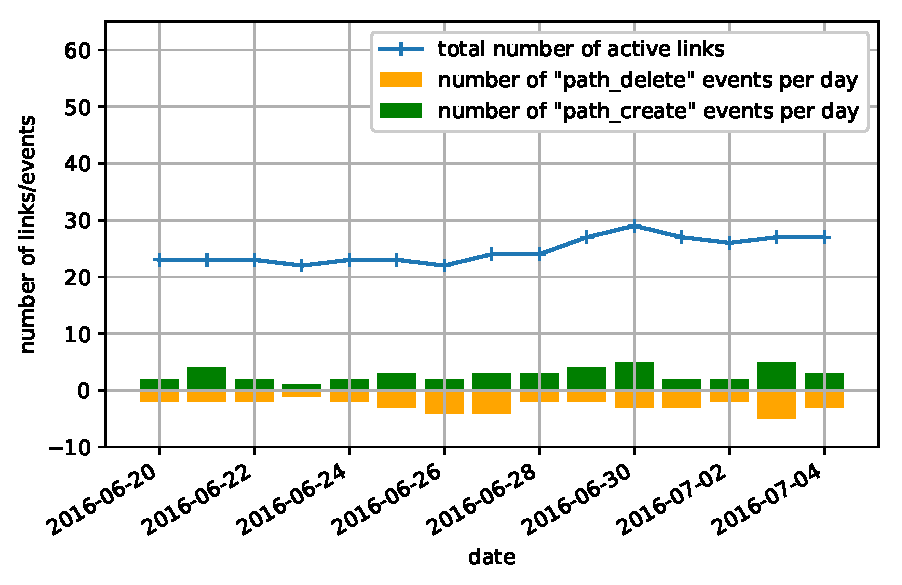
\includegraphics[width=\columnwidth]{net_churn_agri.eps}
        \caption{\agri}
    \end{subfigure}
    \begin{subfigure}[h]{0.49\textwidth}
        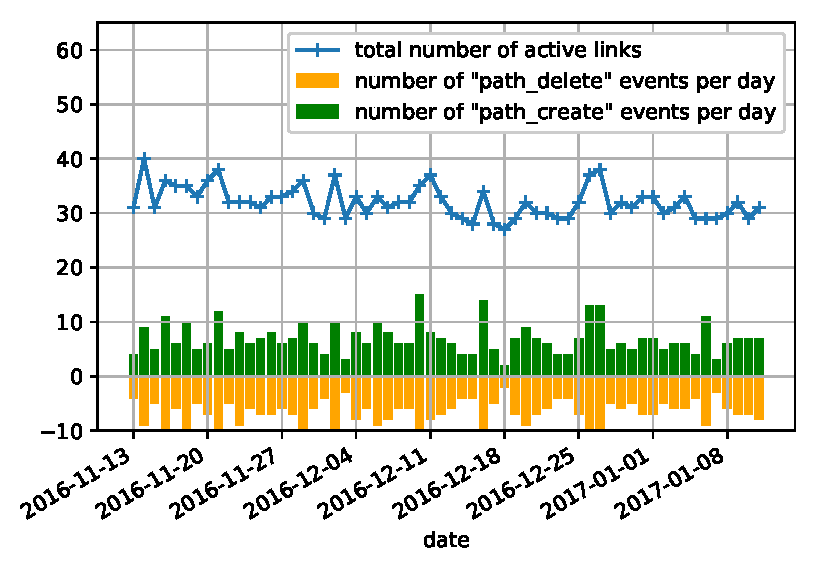
\includegraphics[width=\columnwidth]{net_churn_building.eps}
        \caption{\building}
    \end{subfigure}    
    \caption{
        Network stability: the number of \pathcreate and \pathdelete events generated per day over a 16 days (\agri) and two months (\building).
        The top line shows the total number of active links.
    }
    \label{fig:net_churn}
\end{figure}

% discussion

This stability can largely be attributed to the use of channel hopping.
Changing frequency for each frame is known to efficiently combat multi-path fading and external interference~\cite{watteyne09reliability}, the major causes of instability.
It does not contradict the findings of~\cite{srinivasan08beta}, it just means that link-layer retransmissions can efficiently cope with link burstiness, and that the multi-hop topology can remain very stable.

%==============================================================================
\section{Conclusion}
\label{sec:conclusion}

% intro

This article analyzes the network statistics generated by two low-power wireless mesh networks deployed in real-world conditions.
The first network is deployed in a peach orchard in Argentina, in a \agri scenario.
Its 21~motes have produced \PEACHNUMSTATS~statistic measurements over the course of 3~months.
The second network is deployed in an office building in Paris, in a \building scenario.
Its 17~motes have produced \EVANUMSTATS~statistic measurements over the course of 3~months.

% intuitive

We use a ``waterfall'' plot to show that the two networks are subject to different amounts of external interference from other wireless devices deployed in the same area.
The \smip network delivers its exceptional performance, with 0~packets lost out of \PEACHNUMPCKTS (\agri) and \EVANUMPCKTS (\building) received (100\% reliable) and 4-8 years of battery lifetime on a pair of commercial AA batteries.
This is representative of the performance of 6TiSCH technology.

% non-intuitive

While it is often assumed that wireless links are asymmetric, we show to the contrary that the difference in RSSI averaged over 15~IEEE802.15.4 channels does not exceed a handful of dB.
We show that the network is extremely stable, with less than 5~links being added or deleted per day in the \agri deployment, less than 15 in the \building deployment.
We attribute this performance to the use of Time Synchronized Channel Hopping (TSCH) technology at the heart of the \smip products.

% conclusion

We conclude that \smip is a perfectly suitable IoT solution for \agri and \building applications.

%==============================================================================
\section*{Acknowledgments}

This work was partially supported by
the STIC-AmSud program through the PEACH project,
the Dust Networks Product Group at Analog Devices,
the European Commission through the H2020~F-Interop and H2020~ARMOUR projects,
Inria through the REALMS and DIVERSITY associate teams,
and the Spanish Ministry of Economy and the FEDER regional development fund through the SINERGIA project (TEC2015-71303-R).

%==============================================================================
\section*{References}
\bibliographystyle{elsarticle-num}
\bibliography{brun17using}

\end{document}
